%!TEX root = final.tex
\subsection{Analyzing the Effect of Bail on the Probability to Plea}
\subsubsection{All Else Equal --- Random Forest}
We first carry out the All Else Equal analysis through a Random Forest model.
Appendix \ref{appendixA} shows the calibration information for the Random Forest models for both
Non--Quality of Life and
Quality of Life cases.
We observe that the models are accurate and serviceable,
though the Non--QoL model consistently over--predicts the probability of pleading in the unaltered test set.

Tables~\ref{table:non--QoL_plead} and
       \ref{table:QoL_plead},
respectively,
include the mean predicted probability of pleading at different burden levels for
Non--Quality of Life and
Quality of Life cases, respectively.
Figures~\ref{fig:non--QoL_plead} and
        \ref{fig:QoL_plead}, show the CDFs of same values determined through the model.
Applying the GLM to the dataset reveals roughly similar predictions, as illustrated by
Figures~\ref{fig:non--QoL_plead_GLM} and
        \ref{fig:QoL_plead_GLM}.


We observe that,
especially for Non--Quality of Life cases,
jailing someone substantively increases the predicted probability of pleading when compared other burden levels.
This effect can be observed through both the higher means and the right--shift on the CDF plots.
The effect is similar, though much less pronounced, for Quality of Life cases.

\begin{table}
\centering
\begin{tabular}{|p{0.3\textwidth}|p{0.6\textwidth}|}
  \hline
\textbf{Burden Level} & \textbf{Mean Predicted Probability of Pleading} \\ \hline
    ROR & 0.3631537 \\ \hline
    Trivial & 0.3834242 \\ \hline
    Delay & 0.3744825 \\ \hline
    Jail & 698843  \\ \hline
  \end{tabular}
  \caption{Mean Probability of Pleading for Non--Quality of Life offenses through All Else Equal Analysis using Random Forest model}
  \label{table:non--QoL_plead}
\end{table}

\begin{table}
\centering
\begin{tabular}{|p{0.3\textwidth}|p{0.6\textwidth}|}
  \hline
\textbf{Burden Level} & \textbf{Mean Predicted Probability of Pleading} \\ \hline
    ROR & 0.6072936 \\ \hline
    Trivial & 0.6102411 \\ \hline
    Delay & 0.5999771 \\ \hline
    Jail & 0.648984 \\ \hline
  \end{tabular}
  \caption{Mean Probability of Pleading for Quality of Life offenses through All Else Equal Analysis using Random Forest model}
  \label{table:QoL_plead}
\end{table}


\begin{figure}[t!]
  \centering
  \begin{subfigure}[b]{0.49\textwidth}
    \caption{Non--Quality of Life cases}
    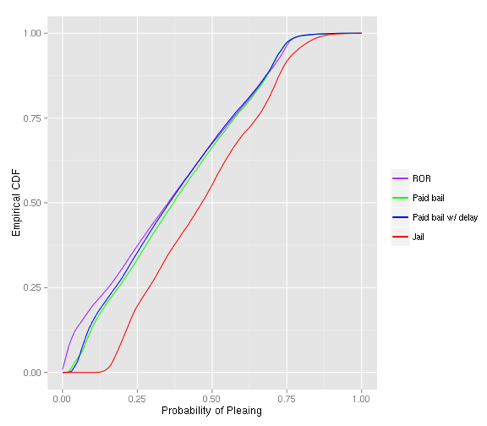
\includegraphics[width=\textwidth]{figures/figx.png}
    \label{fig:non--QoL_plead}
  \end{subfigure}
  ~
  \begin{subfigure}[b]{0.49\textwidth}
    \caption{Quality of Life cases}
    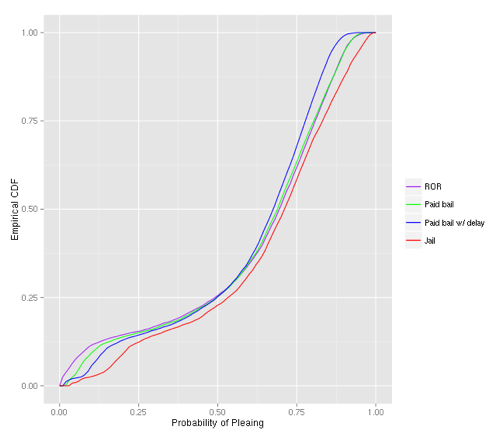
\includegraphics[width=\textwidth]{figures/figy.png}
    \label{fig:QoL_plead}
  \end{subfigure}
  \caption{CDFs of predicted probability of pleading guilty at different burden levels
           determined through the All Else Equal Random Forest model}
  \begin{subfigure}[b]{0.49\textwidth}
    \caption{Non--Quality of Life cases}
    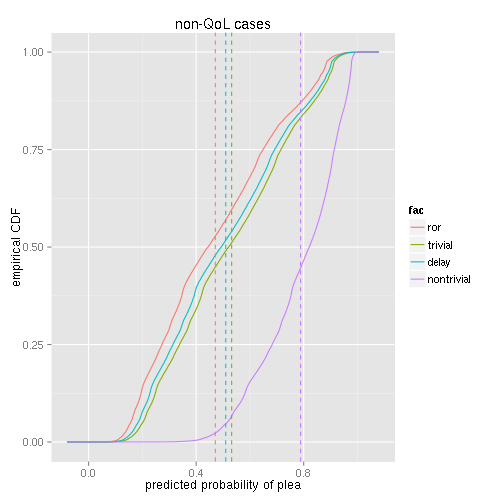
\includegraphics[width=\textwidth]{figures/glmplots/plea_cdf.png}
    \label{fig:non--QoL_plead_GLM}
  \end{subfigure}
  ~
  \begin{subfigure}[b]{0.49\textwidth}
    \caption{Quality of Life cases}
    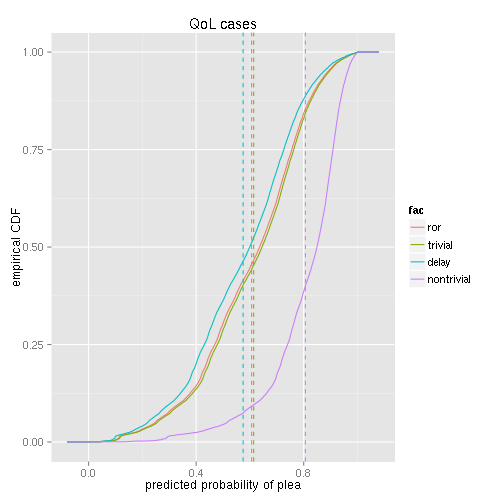
\includegraphics[width=\textwidth]{figures/glmplots/pleaq_cdf.png}
    \label{fig:QoL_plead_GLM}
  \end{subfigure}
  \caption{CDFs of predicted probability of pleading guilty at different burden levels
           determined through the Generalized Linear Model}
\end{figure}


\subsubsection{Propensity Score Matching --- Random Forest}
Finally, we carry out the Propensity Score analysis through a Random Forest model.
Appendix \ref{appendixA}
also includes the calibration information for the Random Forest models to predict ROR for each type of case.
We observe that the ROR prediction models are accurate and unbiased.

Tables \ref{table:ROR_non--QoL_propensity_score} and
       \ref{table:ROR_QoL_propensity_score},
respectively, include the mean predicted probability of pleading for
  ROR and Non--ROR, for
  Non--Quality of Life and Quality of Life cases,
  respectively.
Figures~\ref{fig:ROR_non--QoL_propensity_score} and
        \ref{fig:ROR_QoL_propensity_score} show
the CDFs of same values determined through the model
(also see findings through GLM approach in
Figures~\ref{fig:ROR_non--QoL_GLM} and
        \ref{fig:ROR_QoL_GLM}).


Our results match the All Else Equal analysis.
Especially for Non--Quality of Life cases, a Non--ROR burden level increases the predicted probability of pleading.
Future work should repeat this analysis using
Jail and
Non--Jail burden levels,
as those levels are where the substantive difference occurs in the All Else Equal analysis.


\begin{table}
\centering
  \begin{tabular}{|p{0.3\textwidth}|p{0.6\textwidth}|}
    \hline
    \textbf{Burden Level} & \textbf{Mean Predicted Probability of Pleading} \\ \hline
    ROR & 0.3706164 \\ \hline
    Non--ROR & 0.412566 \\ \hline
  \end{tabular}
  \caption{Mean Probability of Pleading for Non--Quality of Life offenses through Random Forest Modeling}% Propensity Score Matching}
  \label{table:ROR_non--QoL_propensity_score}
\end{table}


\begin{table}
\centering
  \begin{tabular}{|p{0.3\textwidth}|p{0.6\textwidth}|}
    \hline
    \textbf{Burden Level} & \textbf{Mean Predicted Probability of Pleading} \\ \hline
    ROR & 0.6127946 \\ \hline
    Non--ROR & 0.6363191 \\ \hline
  \end{tabular}
  \caption{Mean Probability of Pleading for Quality of Life offenses through Random Forest Modeling}% Propensity Score Matching}
  \label{table:ROR_QoL_propensity_score}
\end{table}


\begin{figure}
  \centering
  \begin{subfigure}[b]{0.49\textwidth}
    \caption{Non--Quality of Life cases}
    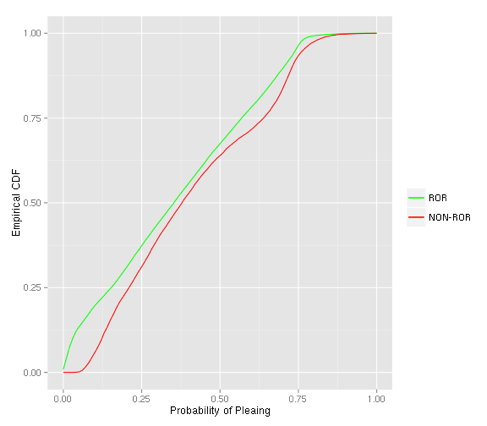
\includegraphics[width=\textwidth]{figures/figxx.png}
    \label{fig:ROR_non--QoL_propensity_score}
  \end{subfigure}
  ~
  \begin{subfigure}[b]{0.49\textwidth}
    \caption{Quality of Life cases}
    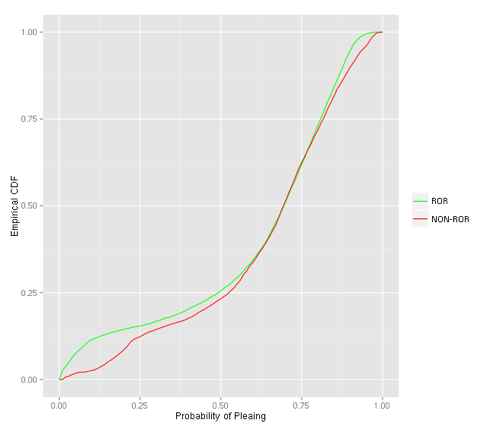
\includegraphics[width=\textwidth]{figures/figyy.png}
    \label{fig:ROR_QoL_propensity_score}
  \end{subfigure}
  \caption{CDFs for the mean predicted probability of pleading for ROR and non--ROR through Random Forest Modeling}% Propensity Score Matching}
  \begin{subfigure}[b]{0.49\textwidth}
    \caption{Non--Quality of Life cases}
    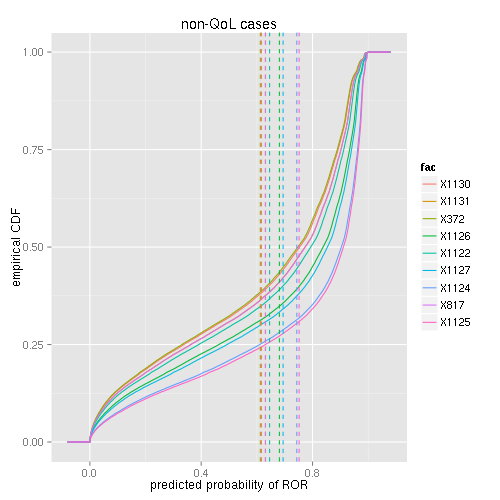
\includegraphics[width=\textwidth]{figures/glmplots/ror_cdf.png}
    \label{fig:ROR_non--QoL_GLM}
  \end{subfigure}
  ~
  \begin{subfigure}[b]{0.49\textwidth}
    \caption{Quality of Life cases}
    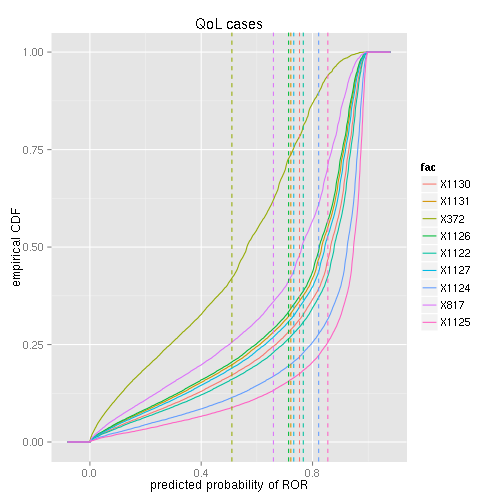
\includegraphics[width=\textwidth]{figures/glmplots/rorq_cdf.png}
    \label{fig:ROR_QoL_GLM}
  \end{subfigure}
  \caption{CDFs for the mean predicted probability of pleading for ROR and non--ROR through Generalized Linear Model}
\end{figure}


\begin{figure}
  \centering
  \begin{subfigure}{0.49\textwidth}
    \caption{Non--Quality of Life cases}
    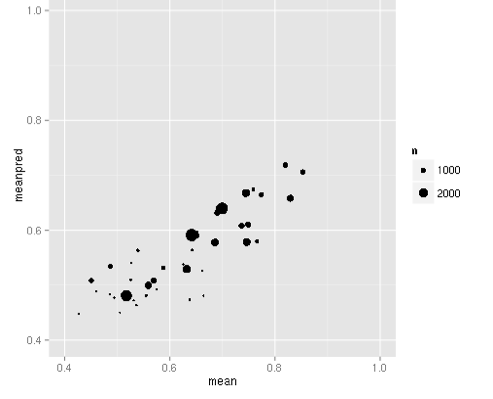
\includegraphics[width=\textwidth]{figures/figaa.png}
    \label{fig:mean_ROR_non--QoL}
  \end{subfigure}
  ~
  \begin{subfigure}{0.49\textwidth}
    \caption{Quality of Life cases}
    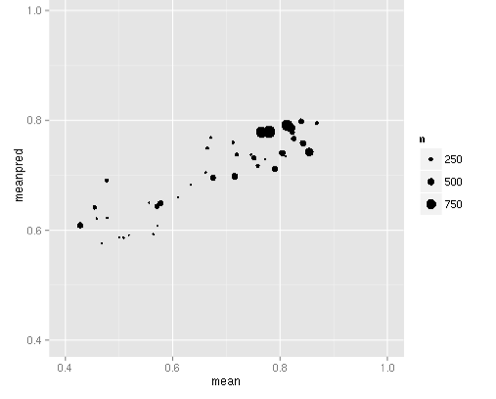
\includegraphics[width=\textwidth]{figures/figbb.png}
    \label{fig:mean_ROR_QoL}
  \end{subfigure}
  \caption{mean probability of ROR for each judge, vs.
  actual percentage of ROR modeled by Random Forest}

  \begin{subfigure}{0.49\textwidth}
    \caption{Non--Quality of Life cases}
    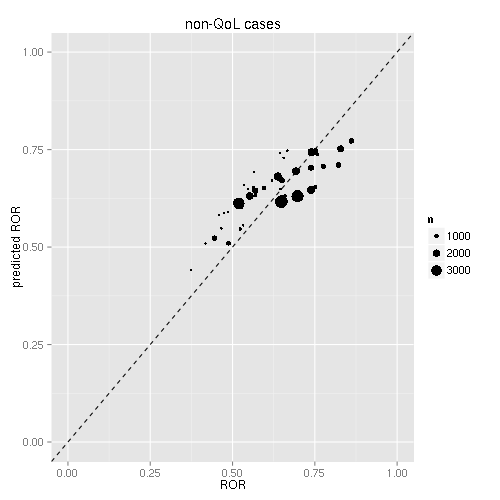
\includegraphics[width=\textwidth]{figures/glmplots/ror_scatter.png}
    \label{fig:mean_ROR_non--QoL_GLM}
  \end{subfigure}
  ~
  \begin{subfigure}{0.49\textwidth}
    \caption{Quality of Life cases}
    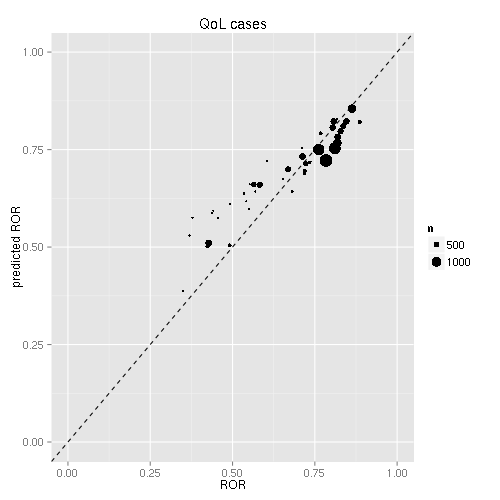
\includegraphics[width=\textwidth]{figures/glmplots/rorq_scatter.png}
    \label{fig:mean_ROR_QoL_GLM}
  \end{subfigure}
  \caption{mean probability of ROR for each judge, vs.
  actual percentage of ROR modeled by GLM}
\end{figure}


\subsection{Analyzing the Effect of Judge on Bail}
Figures~\ref{fig:mean_ROR_non--QoL} and
        \ref{fig:mean_ROR_QoL} show
        the mean predicted probability of ROR
        for each judge versus the judge's actual percentage of ROR,
        for Non--Quality of Life and Quality of Life cases,
respectively.
The plots show that some of the variation in
the judges' percentage of cases that are granted ROR is due to
non--randomness in the cases that they adjudicate.
However,
we observe that for a given mean predicted probability of ROR (on the Y axis),
there is significant judge variance on the true percentage of cases that are granted ROR.
Thus,
this initial analysis shows that different judges do utilize ROR differently for the same types of cases.
As before,
figures~\ref{fig:mean_ROR_non--QoL_GLM} and
        \ref{fig:mean_ROR_QoL_GLM} illustrate similar patterns using a different modeling approach (GLM).